\chapter{Background}\label{chap:background}
This chapter is vital for understanding the following sections of this thesis as it provides some foundational background information in toxicity testing.

\section{Toxicity Testing: From In Vitro Assays and Molecular Fingerprints to Predictive Models and Beyond}\label{sec:toxicity_testing}

With the ever-growing amount of chemical compounds entering the environment, traditional experimentation methods face limitations concerning cost and time constraints. Additionally, ethical concerns arise regarding the use of animal trials in \emph{in vivo} experiments.

In 2007, the \emph{U.S. National Academy of Sciences} introduced a visionary perspective and published a landmark report, titled as \emph{Toxicity Testing in the 21st Century: Vision and Strategy}. This report promoted a transition from conventional, resource-consuming animal-based \emph{in vivo} tests to efficient high-throughput \emph{in vitro} pathway assays on cells. This transition paved the way for the realm of HTS, where a multitude of \emph{in vitro} bioassays can be executed, complementing and improving chemical screening. This transformation is made possible by advancements in robotics, data processing, and automated analysis. As a result, this synergy has led to the generation of extensive toxicity datasets like ToxCast/Tox21.
 
HTS datasets, including ToxCast and other sources, have opened the door to promising applications of machine learning in predictive computational toxicology. These predictive models can be developed to screen environmental samples with limited availability of toxicity data, allowing for the prioritization of further testing efforts. Such models often forecast toxicity using QSARs, which are based on descriptors encoding chemical structures like molecular fingerprints. $1$D-Molecular fingerprints encode compound molecules as fixed-length binary vectors, denoting the presence (1) or absence (0) of specific substructures or functional groups, visualized in~\ref{fig:fingerprint_schema}. Typically, fingerprints use \emph{SMARTS} strings, as an extension of \emph{SMILES} strings, to encode the underlying substructural patterns within molecules. While SMILES is a widely accepted notation system for representing chemical structures, there can be variations in how different sources generate SMILES strings. These variations can include the presence or absence of hydrogens, different ways of representing aromatic rings, variations in chemotypes, and tautomer representations. SMILES strings for the same chemical can differ due to these variations. To ensure consistency and deterministic computation, chemists often normalize SMILES before use, ensuring adherence to a common set of rules for computational analysis.

\begin{figure}
    \centering
    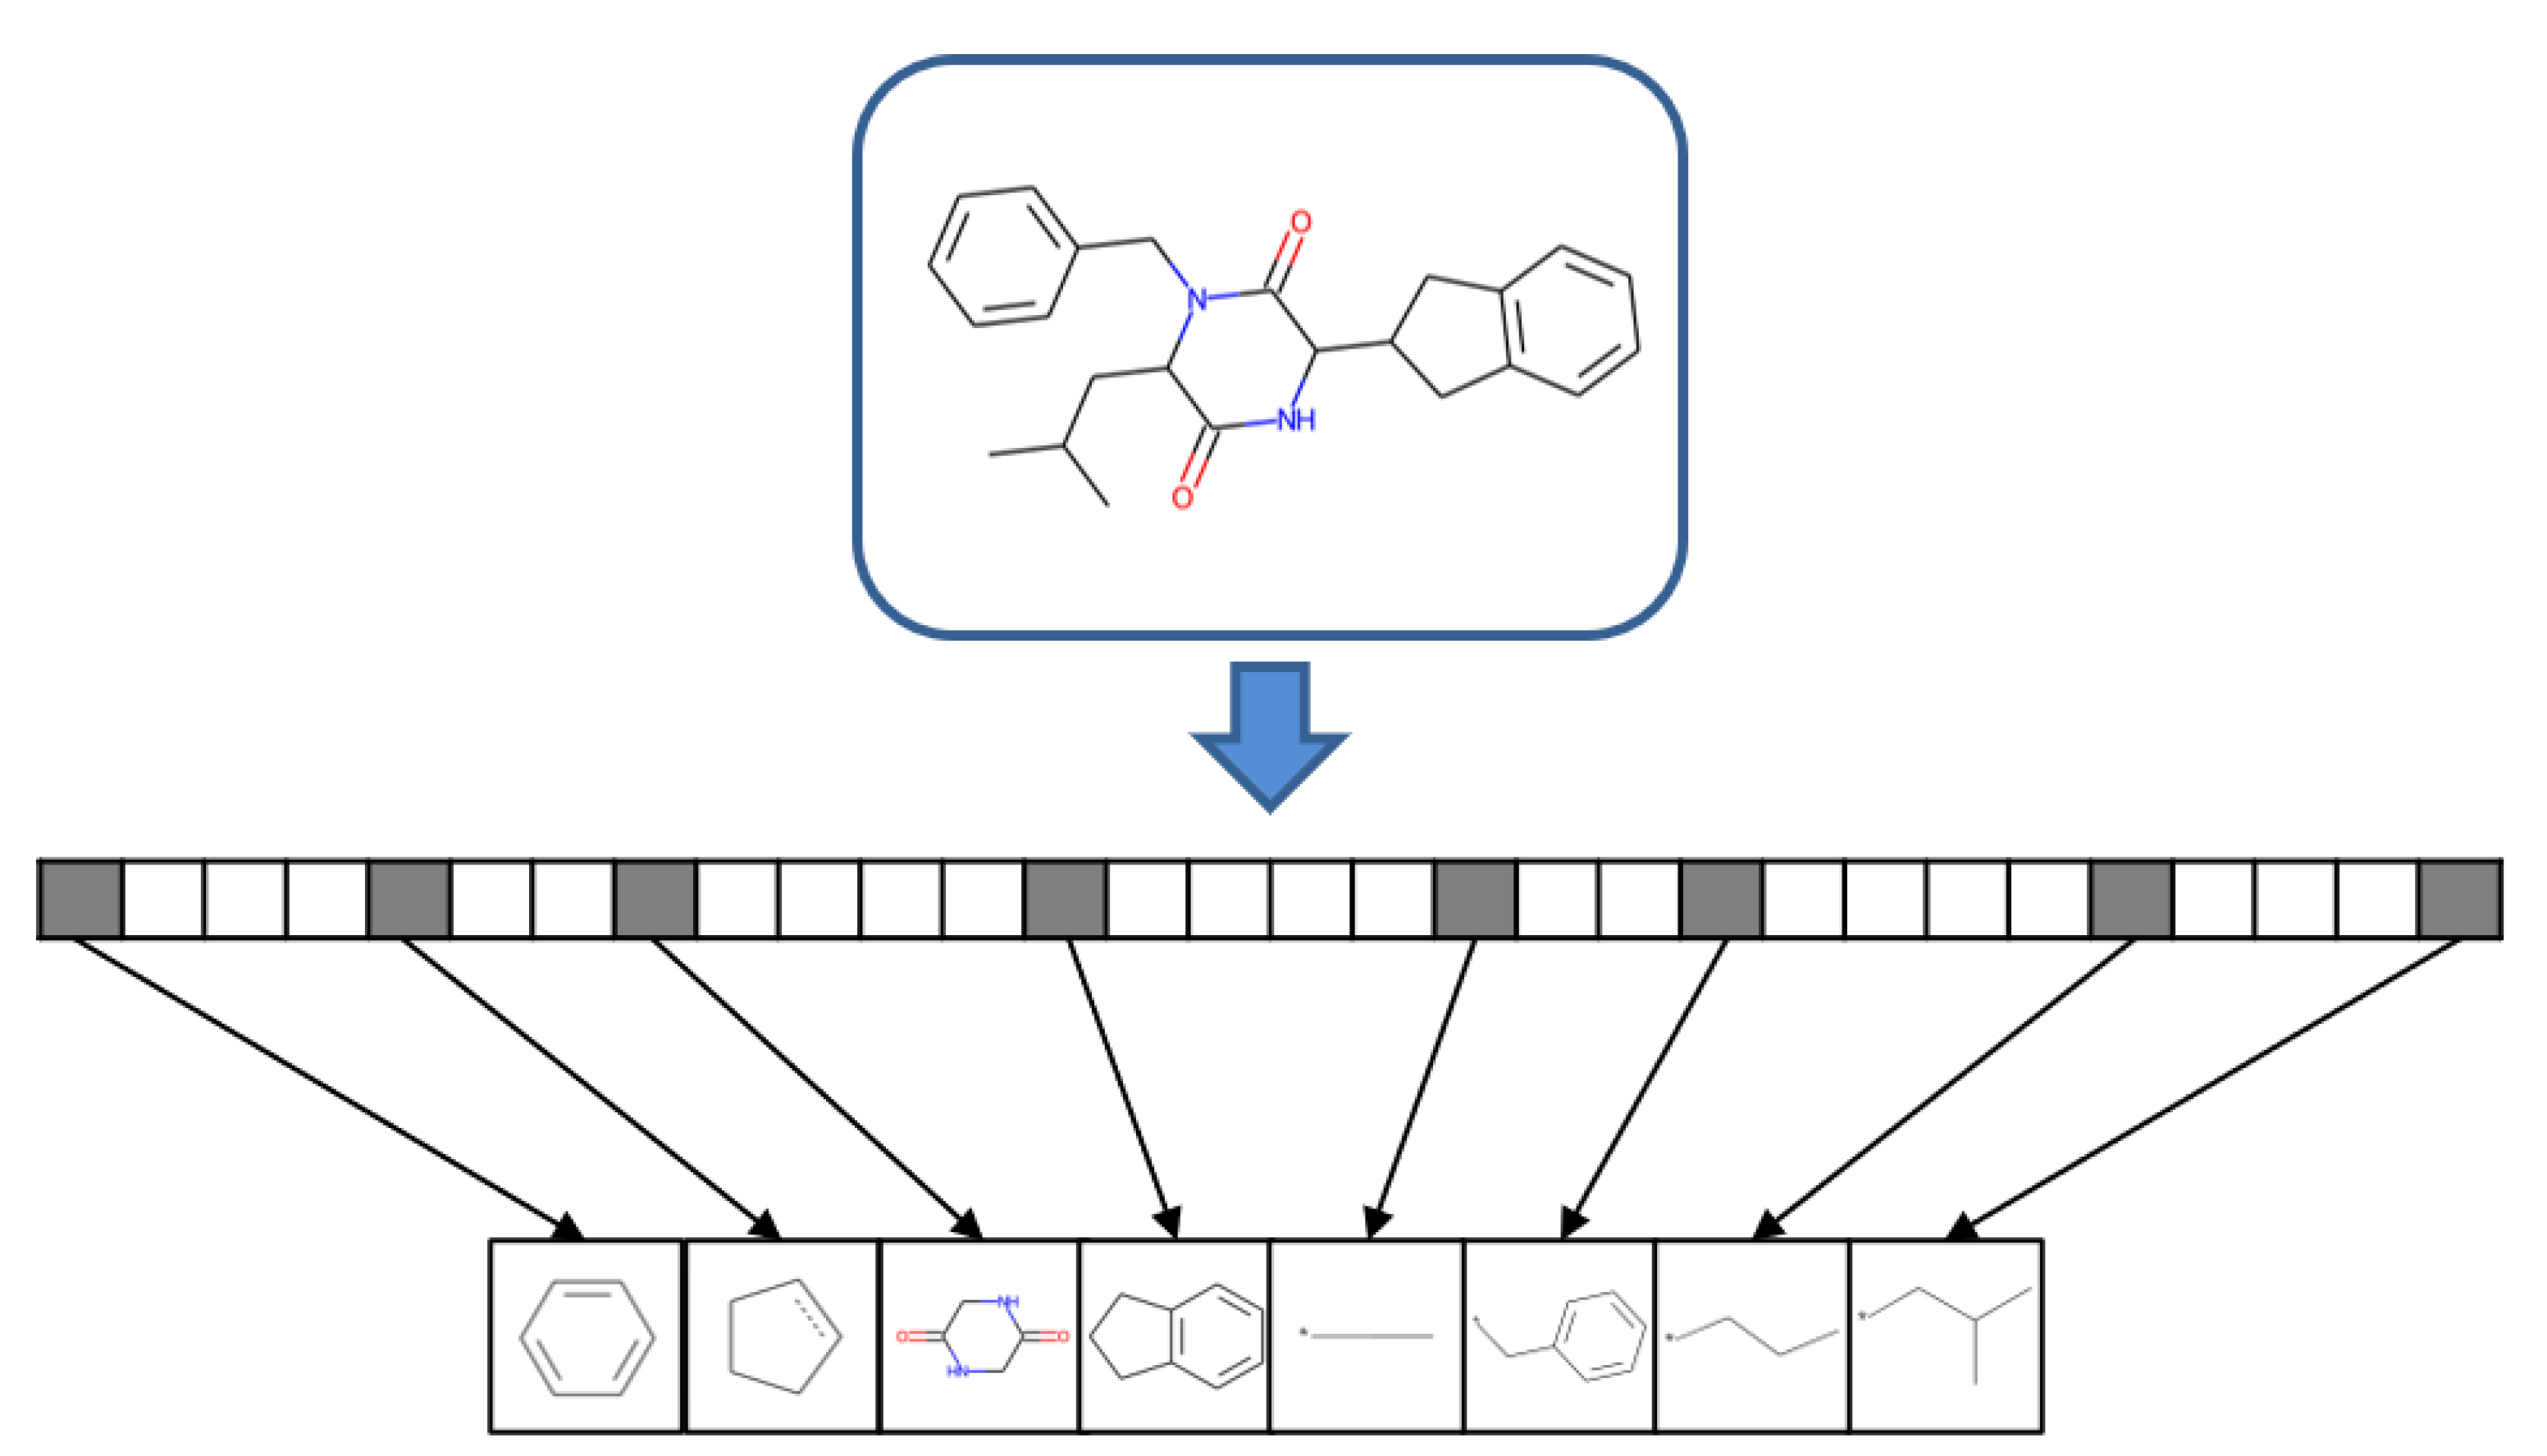
\includegraphics[width=1.0\textwidth]{figures/fingerprint_schema.png}  
    \caption{Schematic of a molecular fingerprint for a fictional chemical. Each bit position accounts for the presence or absence of a specific structural fragment. Bit positions are set on (set to 1, gray) if the substructure is present in a molecule, or set off (set to 0, white) if it is absent. Figure 1 adapted from~\cite{janela2022}.}
~\label{fig:fingerprint_schema} 
\end{figure}

Once generated, molecular fingerprints can be used for various cheminformatics tasks. For example, they can be compared to identify structurally similar compounds, used as input for machine learning models to predict properties or activities.

To go one step further, SIRIUS employs CSI:FingerID, a method that directly predicts various fingerprint types from HRMS/MS fragmentation spectra. CSI:FingerID utilizes machine learning techniques, encompassing linear Support Vector Machines and Deep Learning, to predict an array of fingerprints, including CDK Substructure, PubChem CACTVS, Klekota-Roth, FP3, MACCS, ECFP2, and ECFP4 fingerprints.
% It's important to highlight that CSI:FingerID offers more than just binary predictions. it also provides confidence assessments in the form of Platt probabilities. Moreover, the predicted molecular fingerprints remain valid within the method's predictive capacity, even for compounds not found in any existing database.

The utilization of molecular fingerprints for \emph{in vitro} toxicity prediction is based on the assumption that molecular toxic effects result from interactions between distinct chemical components and receptors during a \emph{molecular initiating event (MIE)}. On a larger biological scale, the MIE can set a sequential chain of causally linked \emph{key events (KE)} in motion. This occurs at different levels of biological organization from within cells to potentially culminating in an \emph{adverse outcome pathway (AOP)} at the organ or organism level, as depicted in Figure~\ref{fig:aop}. The mechanistic information captured in AOPs reveal how chemicals or other stressors cause harm, offering insights into disrupted biological processes, potential intervention points but also guide regulatory decisions on next generation risk assessment and toxicity testing. The AOP framework is an analytical construct that allows an activity mapping from the presence or absence of certain molecular substructures encoded in chemical descriptors to the target mechanistic toxicity. Finally, when monitoring disruptions in toxicity pathways, physiologically based pharmacokinetic (PBPK) models can be leveraged to extrapolate \emph{in vitro} findings to human blood and tissue concentrations~\cite{bell2018}.

It is important to emphasize that the predictions from HTS bioassays portray molecular toxicity events only at a cellular level, and their translation to adverse outcomes at higher organism levels is not necessarily guaranteed. As the scale shifts from the cellular to the organism level, the confidence in these relationships may decrease.

\begin{figure}[htbp]  % Placement options: h (here), t (top), b (bottom), p (page)
    \centering
    \includegraphics[width=1.0\textwidth]{figures/aop2.png}  
    \caption{Diagram of (A) an adverse outcome pathway (AOP) and (B) an AOP network. (A) An AOP starts with a molecular initiating event (MIE), followed by a series of key events (KEs) on different levels of biological organization (cellular, tissue, organ) and ends with an adverse outcome (AO) in an organism. The stressor is not part of the AOP itself. Figure 1 adapted from~\cite{nymark2021}}
~\label{fig:aop} 
\end{figure}


\section{Chemical Target Toxicity vs. Cytotoxicity}\label{sec:cytotoxicity}

Consider a hypothetical scenario in which a chemical undergoes testing in a bioassay that assesses toxicity by measuring the activation of a reporter gene within a cell. The reporter gene encodes a detectable protein, and its activation is triggered by the chemical binding to a specific receptor, the key focus of the assay endpoint. While it might seem logical that an increase in chemical concentration would result in a higher chemical toxicity signal, this assumption does not hold true in general. At elevated concentrations, the chemical can become \emph{cytotoxic}, causing harm to the cells and ultimately leading to cell death. Consequently, this can lead to a decrease in the activation of the reporter gene and a subsequent reduction in the signal, indicating a decrease in bioactivity. For a visual representation, consult Figure~\ref{fig:cytotoxicity}. Considering this situation, chemical toxicity can manifest in various forms, categorizing into two primary groups~\cite{judson2016}: 
\begin{itemize}
    \item \textbf{Specific toxicity} occurs when a chemical interacts with and interferes with a specific biomolecular target or pathway, manifesting as effects like receptor agonism/antagonism or enzyme activation/inhibition. This thesis primarily focuses on specific toxicity, which is often the desired signal to detect in a target assay endpoint. However, it is essential to recognize that data processing must also take into account the following:
    \item \textbf{Non-specific toxicity (Cytotoxicity and cell stress)} involve broad disruptions of the cellular machinery, including reactions with DNA as well as processes like apoptosis, oxidative stress and mitochondrial disturbance. Cell viability can be evaluated either individually or concurrently with the target bioassay endpoint. For instance, one approach involves evaluating the cell viability by determining the proportion of live cells within a population. This is achieved using a fluorescent dye that selectively enters living cells, as it cannot permeate the membranes of deceased cells, resulting in fluorescence intensity directly reflecting cell viability.
\end{itemize}

\begin{figure}[htbp]  % Placement options: h (here), t (top), b (bottom), p (page)
    \centering
    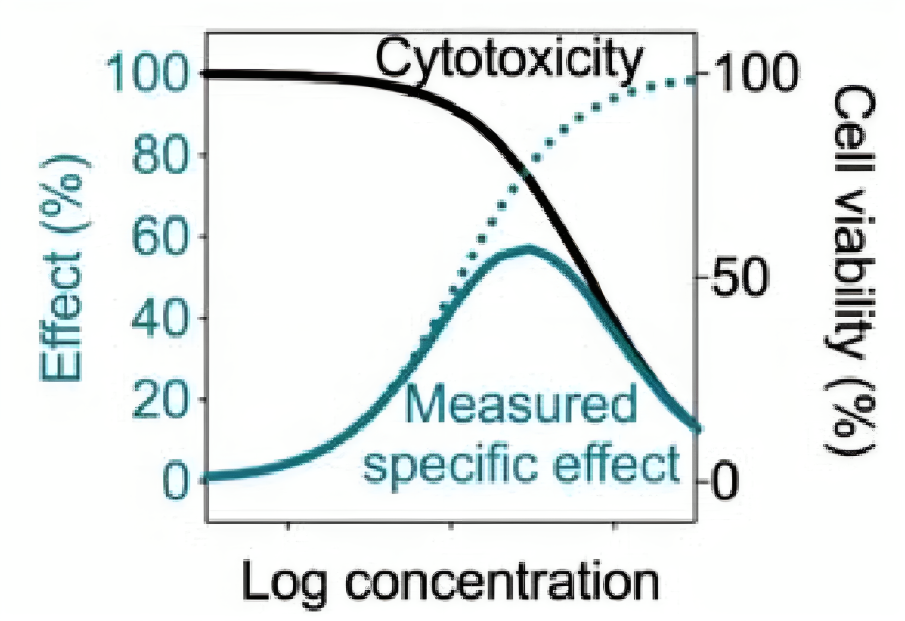
\includegraphics[width=0.55\textwidth]{figures/cytotoxicity.png}  
    \caption{Example of a bioassay response with cytotoxicity interference. The dotted line shows the theoretical specific toxicity effect but due to non-specific cytotoxicity (black line is cell viability), the measured effect may have an inverted U-shape within the tested concentration range. The measured specific effect may also be influenced by the presence of the cytotoxicity burst phenomenon, which can lead to a non-specific exponential growth phase before the subsequent decline in the effect curve. Figure 7.8 from~\cite{escher2021}.}
~\label{fig:cytotoxicity} 
\end{figure}

An associated phenomenon is referred to as the \emph{cytotoxicity burst}~\cite{judson2016}, in which the expected specific toxicity interferes with non-specific cellular stress responses that may become overly activated within a critical range of toxicant concentration. As the concentration of the toxic substance approaches levels that induce cell death, the signal associated with the presumably specific toxicity of a target assay endpoint becomes increasingly mixed with signals stemming from non-specific responses~\cite{escher2021}. Only from the observed responses of the target assay endpoint it can not be deduced what are the specific and non-specific shares in the measured signal.

Referred to as~\emph{false positive} hitcalls, these are associated with compounds where the activity response surpasses the efficacy cutoff mainly because of non-specific toxicity. Nevertheless, in many research contexts, there exists a particular interest in pinpointing specific toxicity~\cite{fay2018}. This becomes crucial for identifying the molecular initiating event and understanding the adverse outcome pathway. Solely based on the observed signal, the challenge arises in differentiating true positives, where the compound exhibits specific toxicity without cytotoxicity interference, from false positive hitcalls. This introduces significant uncertainty in the reported activity hitcalls.

Nonetheless, the ToxCast pipeline is deliberately structured to minimize the occurrence of \emph{false negative} hitcalls. The original pipeline employs a fairly inclusive risk assessment approach, ensuring that compounds with ambiguous toxicity potential are more likely to be rated as active rather than inactive. Moreover, the toxicity assessment process within this pipeline lacks proper mechanisms to differentiate between activity arising from specific and non-specific chemical toxicity.

Although not the central emphasis of this study, we investigate the possibility of reducing potential overestimation of positive hitcalls attributed to suspected non-specific components in the reported activity. This is achieved by comparing potency concentrations between the target assay endpoints and the corresponding viability or burst assay endpoints, which quantify cytotoxic cell loss or cell stress, respectively. If the probabilities indicate that a crucial potency concentration from the cytotoxicity assay endpoint is lower than that of the target assay endpoint, previously identified false positive hitcalls can be reduced by a factor reflecting the potential impact of cytotoxicity interference.






